% This is samplepaper.tex, a sample chapter demonstrating the
% LLNCS macro package for Springer Computer Science proceedings;
% Version 2.20 of 2017/10/04
%
\documentclass[runningheads]{llncs}
%
\usepackage{graphicx}

\begin{document}
%
\title{WASP - Windows and Shutters Project}

\author{Group 7: Sebastian Künzel \and
Lukas Nabakowski \and
Jannis Rapp}

\institute{Service Computing Department, IAAS, University of Stuttgart
\email{st150016@stud.uni-stuttgart.de} \and
\email{st148841@stud.uni-stuttgart.de} \and
\email{st150565@stud.uni-stuttgart.de}}
%
\maketitle              % typeset the header of the contribution
%
\begin{abstract}
The abstract should briefly summarize the contents of the report in
150--250 words. 

\keywords{First keyword  \and Second keyword \and Another keyword.}
\end{abstract}
%
%
%
\section{System Introduction}



Quality of Life and well-being is an essential factor for work performance and the health of employees in modern office environments. One prominent problem of indoor office buildings is a high CO$_2$ concentration which lead to impaired work performance and negative health symptoms~\cite{indoor_polutionCO2}. Further possible disturbances in office environments include ambient noise and sunlight~\cite{indoor_noiselight}. Both elements distract the concentration of office workers. 
\newline
We use an intelligent window and shutter management system to address the problems outlined above.
This system uses sensors to monitor the CO$_2$ concentration, ambient noise level, and sunlight intensity.
Based on the observed information, the system can then react by adjusting the windows, shutters, and heating accordingly.
\newline
The goal is to control the office's windows and shutters to maintain high air quality with a low CO$_2$ concentration and a comfortable temperature while avoiding distractions caused by ambient noise and blinding sunlight. The system is also equipped to adapt to environmental influences (e.g. rain and wind) that can adversely affect the indoor office space when windows are open.   




Other weather aspects such, as wind and rain also need to be considered when controlling office windows. Additional, the influence of ambient noise has to be minimized. 




The performance and health of office employees can be increased my monitoring the CO2 concentration, aswell   

To increase the performance and health of employees an automated  



Modern companies are focus




Describe the scope (ghdfghfdhgbackground information and problem statement) and the goals of your project.

Table~\ref{tab1} an example of a table.

\begin{table}
\caption{Table captions should be placed above the
tables.}\label{tab1}
\begin{tabular}{|l|l|}
\hline
Item & Deadline \\
\hline
I111 & D1 \\
I2 & D2 \\
I3 & D3 \\
I4 & D4 \\
I5 & D5 \\
\hline
\end{tabular}
\end{table}

Fig.~\ref{fig1} gives an example of a figure.

\begin{figure}
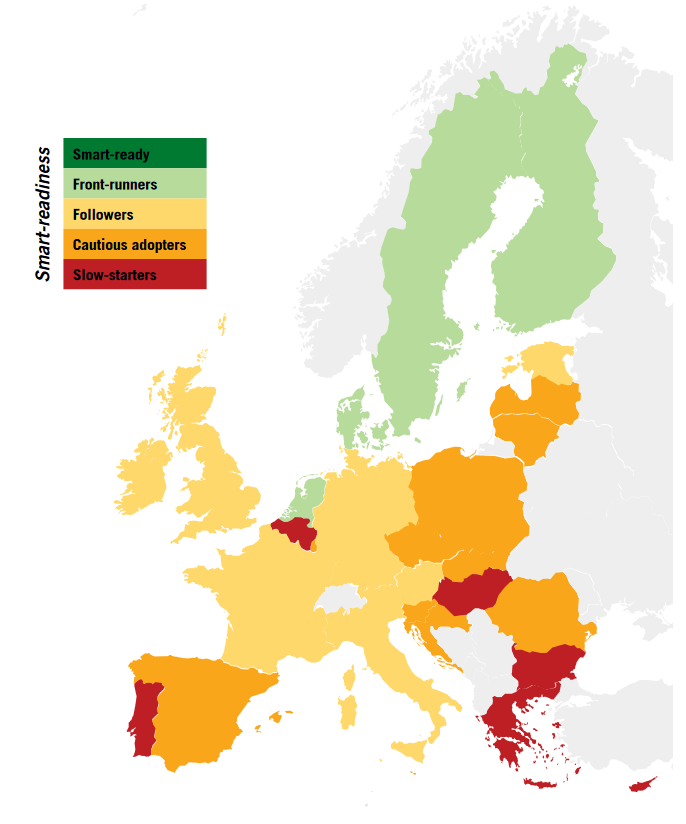
\includegraphics[width=\textwidth]{fig1}
\caption{A figure caption is always placed below the illustration.
Please note that short captions are centered, while long ones are
justified by the macro package automatically.} \label{fig1}
\end{figure}

For citations of references, we prefer the use of square brackets
and consecutive numbers. The following bibliography provides
a sample reference list with entries for journal
articles~\cite{ref_article1}, a book~\cite{ref_book1}, proceedings without editors~\cite{ref_proc1},
and a homepage~\cite{ref_url1}. Multiple citations are grouped
\cite{ref_article1,ref_book1},
\cite{ref_article1,ref_book1,ref_proc1,ref_url1}.

\section{System Analysis}
Describe the user requirements of your system.

\section{System Architecture Design}
Describe and provide a design of the architecture of your system.

\section{System Implementation}
Describe the implementation of your system. This section is only relevant for the report and should be omitted for the project description. 

\section{Discussion and Conclusions}
Here you can discuss some interesting points or limitations of your system and conclude the report.

%
% ---- Bibliography ----
%
\bibliographystyle{splncs04}
\bibliography{mybib}

All links were last followed on April 17, 2020.

\end{document}
